\section{Method}
When performing the naive method of offsetting the outline inward with constant width paths the overfill and underfill problems arise in the center.
Constant widths inward steps might not resolve to the arbitrary width of the outline shape.
Our method therefore decides on the number of beads everywhere first and then determines the widths of the beads.
We decide on a bead count at locations which lie in central positions of the shape in some sense to be defined below and apply an optimal distribution of widths from the central regions outward.

What constitutes an optimal distribution is governed by a beading strategy.
Our framework allows for different beading strategies which can optimize for different criteria.
A beading strategy is defined by several several functions which govern the behavior of our framework.

\begin{enumerate}
\item Compute a skeleton of the outline shape.
\item Use a significance measure to mark regions of the skeleton which are central.
\item Determine the bead count values in the marked regions and handle transitions to different bead count values.
\item Generate junctions along unmarked bones of the skeleton and connect the junctions together to form the extrusion beads.
\end{enumerate}
See \cref{overview_fig}.

\begin{figure}
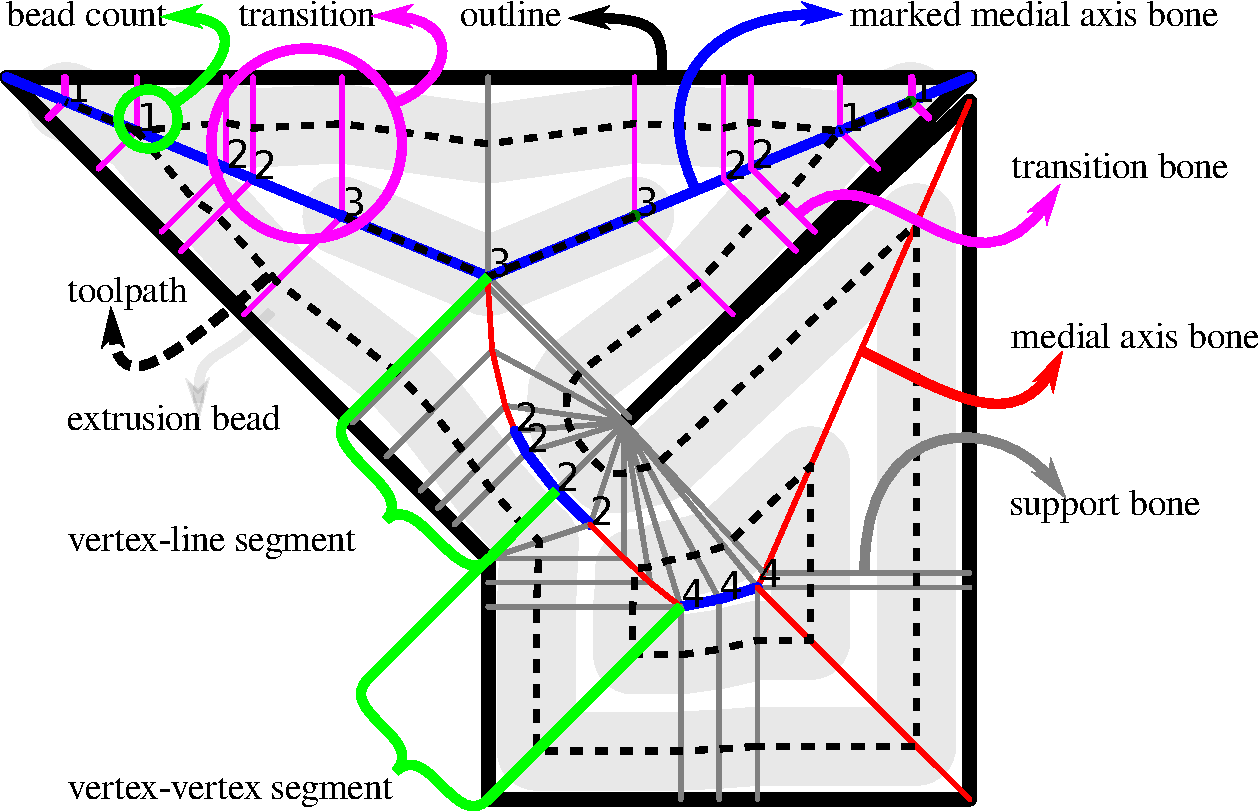
\includegraphics[width=\columnwidth]{sources/method/terminology.pdf}
\caption{Explanation of terms.}
\label{legend}
\end{figure}




\begin{figure*}
\centering
\setlength{\figwidth}{0.19\textwidth}
\begin{subfigure}{\figwidth}
\centering
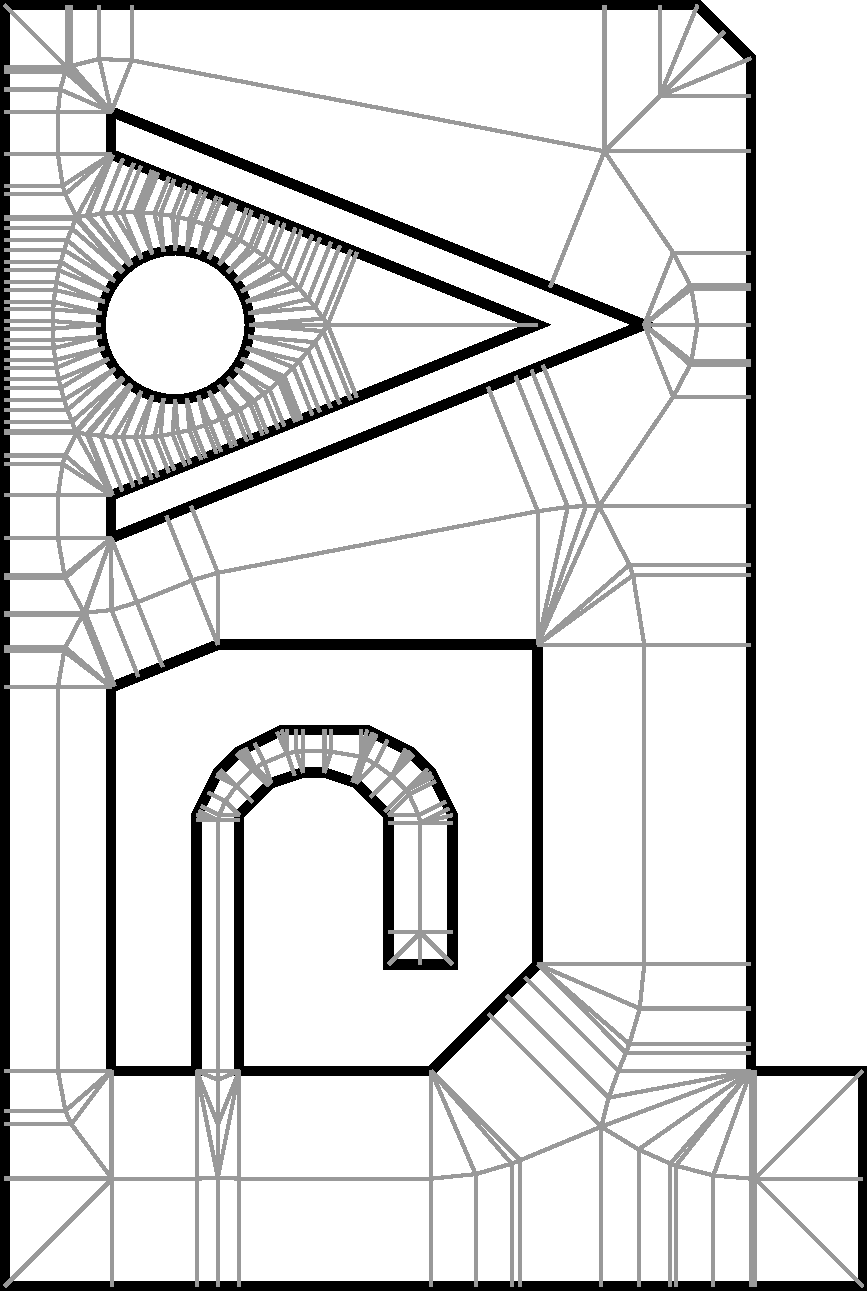
\includegraphics[width=\columnwidth]{sources/method/overview/skeleton.pdf}
\caption{Skeleton}\label{overview_fig_skeleton}
\end{subfigure}
\begin{subfigure}{\figwidth}
\centering
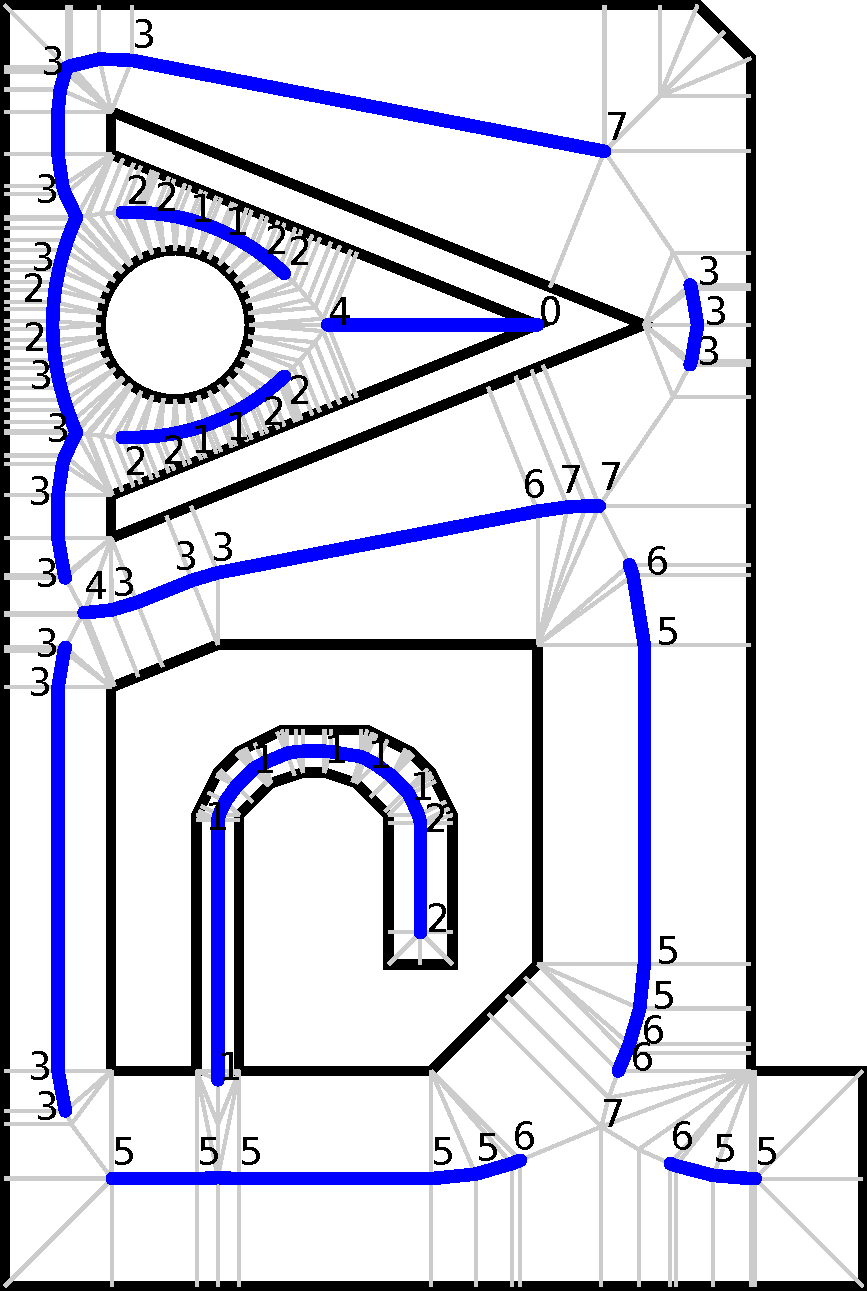
\includegraphics[width=\columnwidth]{sources/method/overview/marked.pdf}
\caption{Marked}\label{overview_fig_marked}
\end{subfigure}
\begin{subfigure}{\figwidth}
\centering
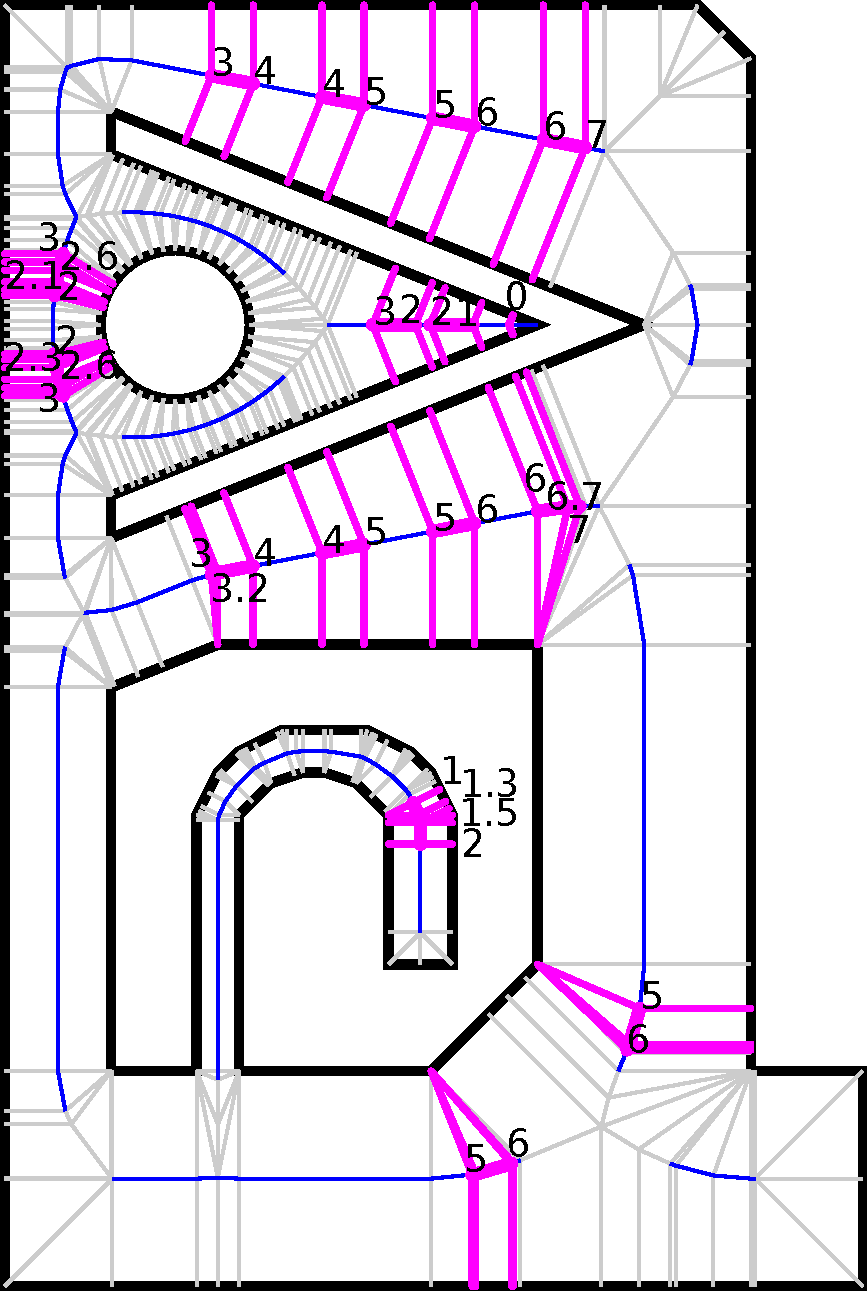
\includegraphics[width=\columnwidth]{sources/method/overview/transitions.pdf}
\caption{Transitions}\label{overview_fig_transitions}
\end{subfigure}
\begin{subfigure}{\figwidth}
\centering
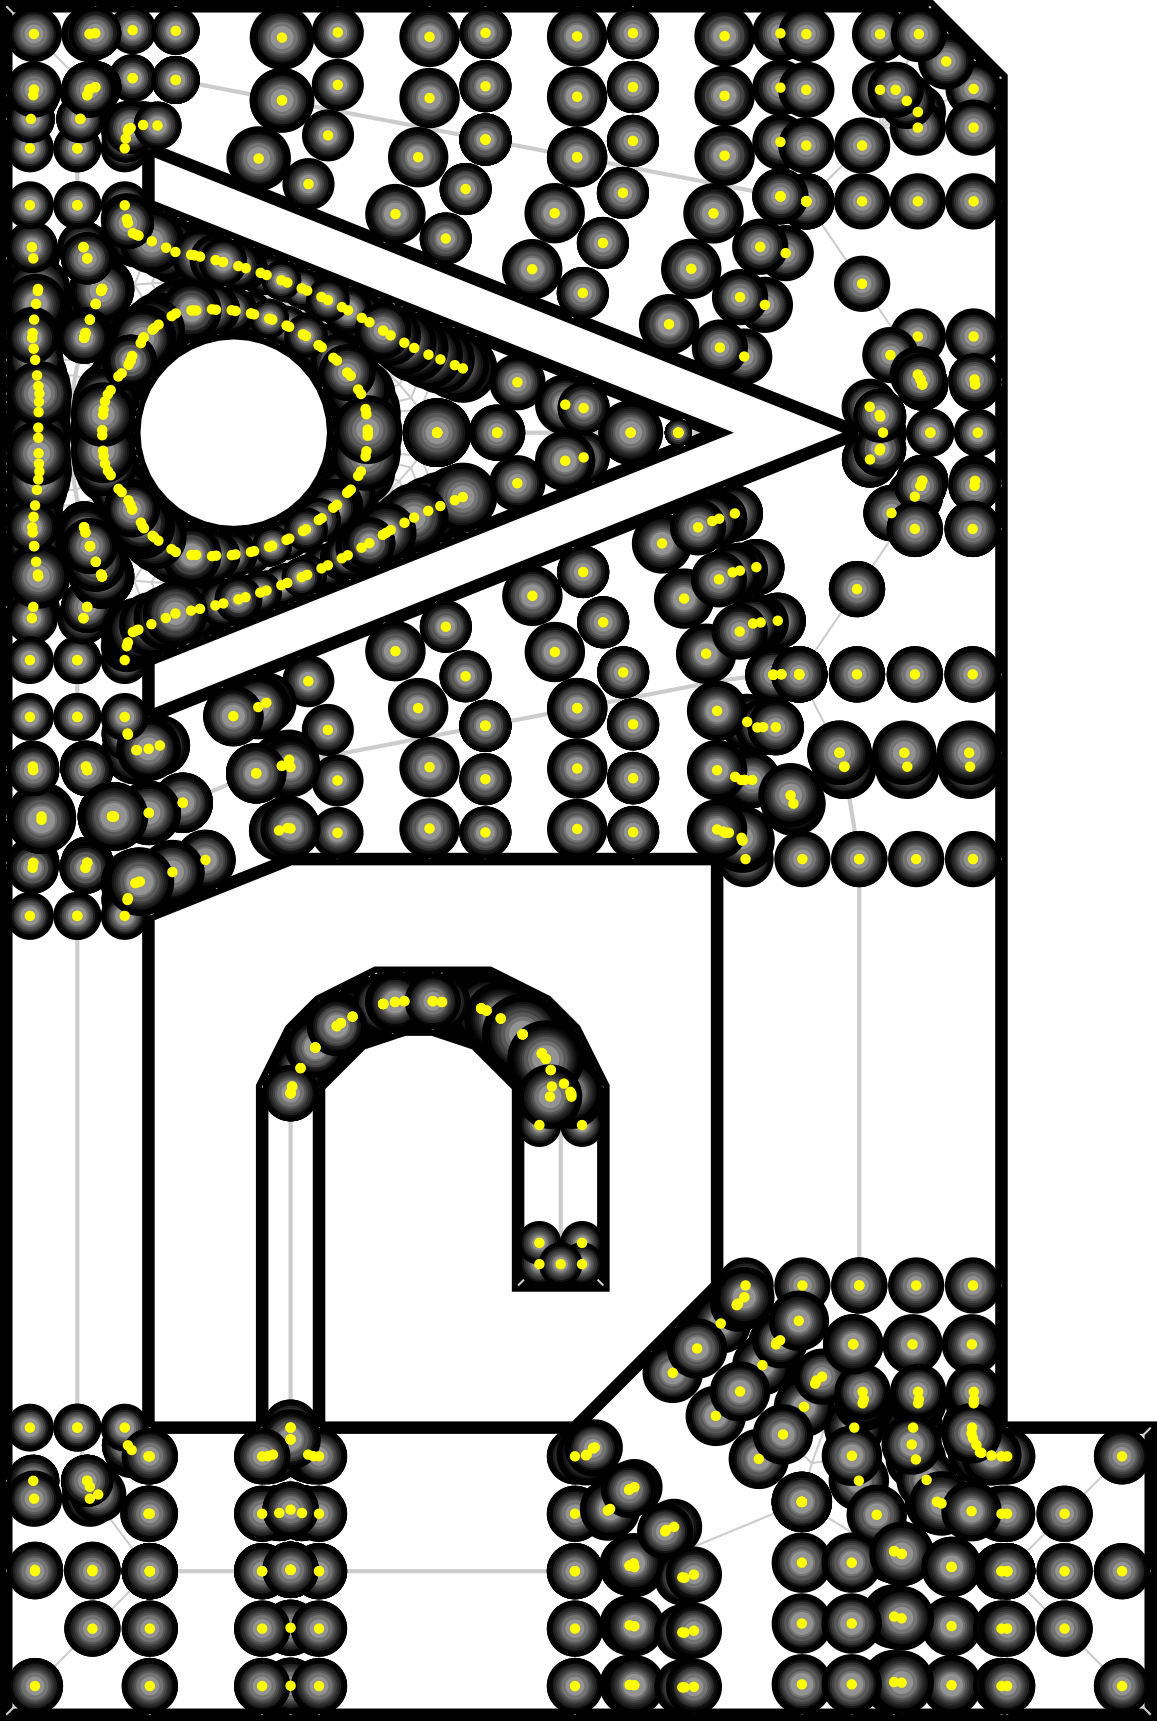
\includegraphics[width=\columnwidth]{sources/method/overview/junctions.png}
\caption{Junctions}\label{overview_fig_junctions}
\end{subfigure}
\begin{subfigure}{\figwidth}
\centering
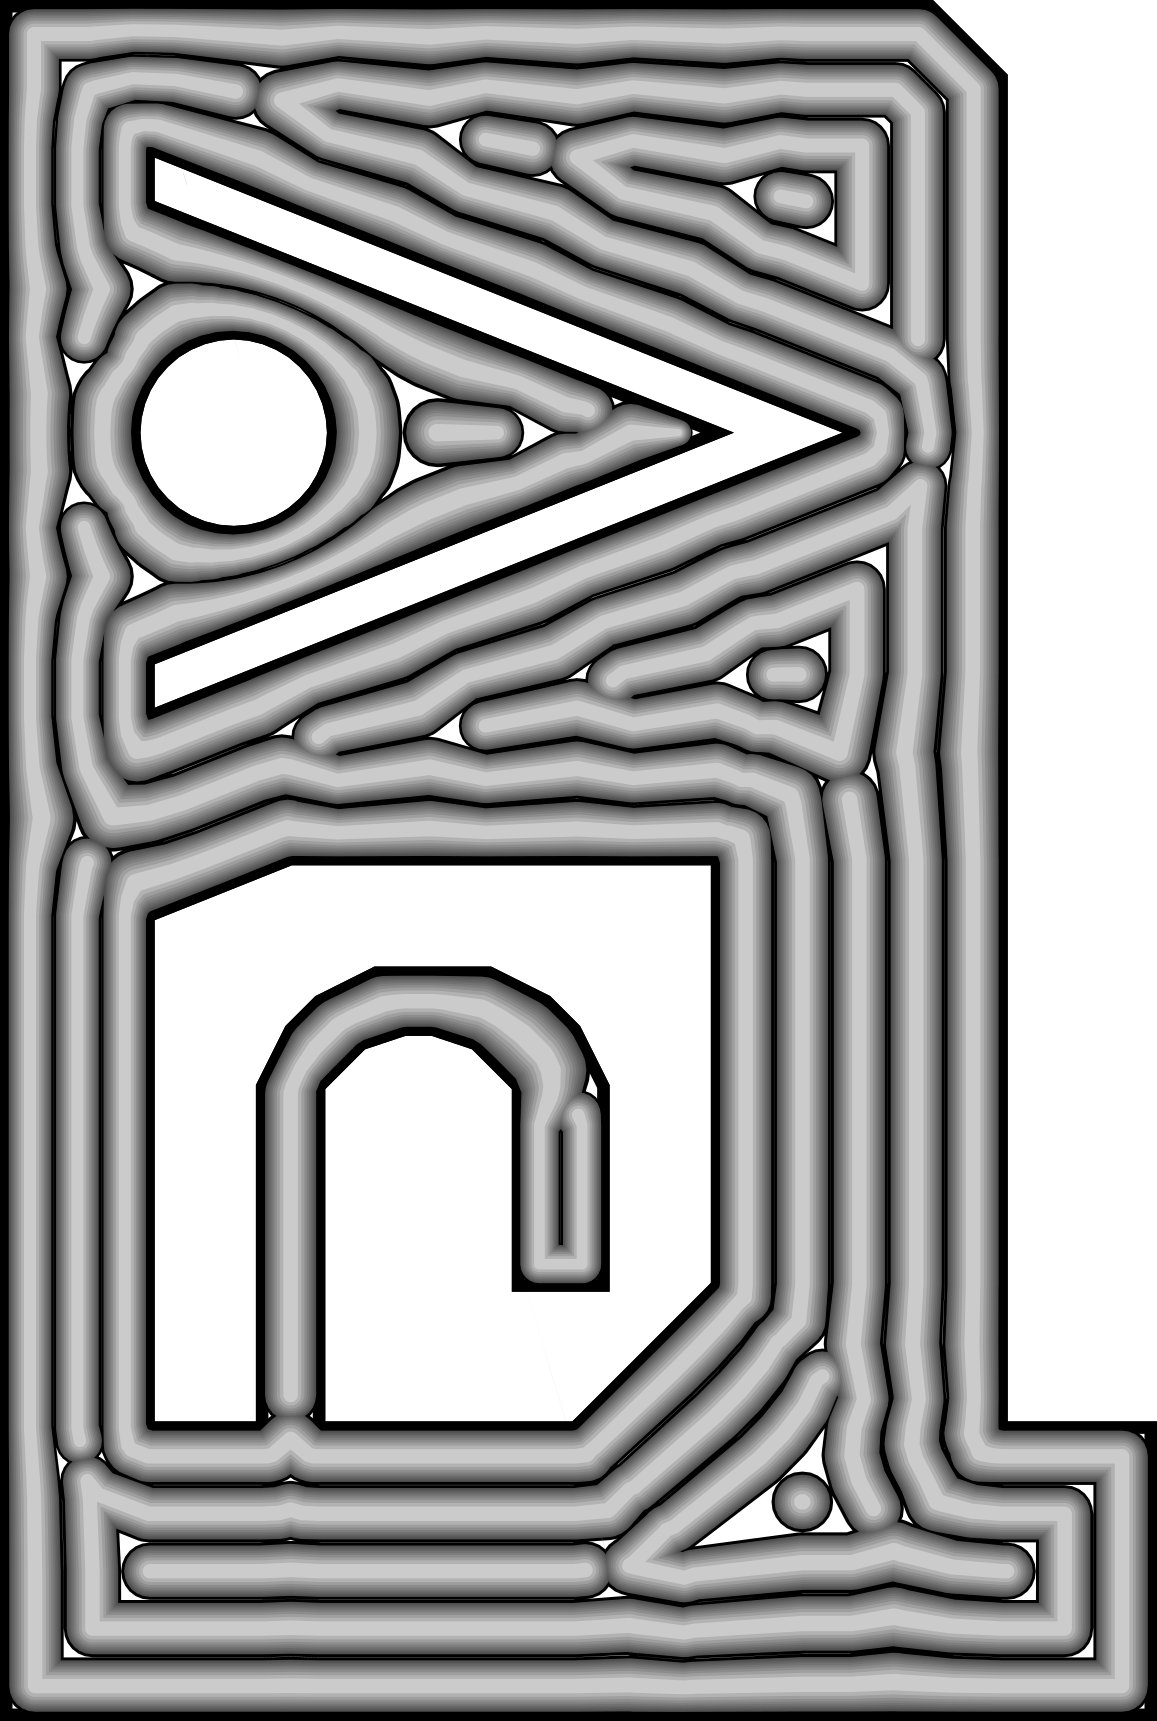
\includegraphics[width=\columnwidth]{sources/method/overview/toolpaths.png}
\caption{Toolpaths}\label{overview_fig_toolpaths}
\end{subfigure}
\caption{
Overview of the steps in the method of our framework.
First we \subref{overview_fig_skeleton} decompose the outline shape into a skeleton (grey), \subref{overview_fig_marked} mark central regions (blue) and determine an initial bead count (numbers) based on the local feature size.
Then we \subref{overview_fig_transitions} make alterations to smoothly transition to a different bead count (magenta).
We then \subref{overview_fig_junctions} generate a number of junctions (yellow) equal to the bead count along the bones of the skeleton,
which are \subref{overview_fig_toolpaths} connected together to make the toolpaths.
}
\label{overview_fig}
\end{figure*}















\subsection{Shape decomposition}
The shape decomposition we employ on the outline shape of a layer is based on a common skeletonization of the polygonal outline shape: the medial axis.
Starting from the medial axis we further decompose the shape into simple fragments, so that we can easily process the shape using piecewise linear approximations.



\subsubsection{Medial axis transform}
One of the most commonly used skeletonizations of a shape is the medial axis.
The medial axis is defined by the locations where the inscribed circle meets the boundary in at least two locations. \cite{blum1967transformation}
We call the set of closest points on the outline polygon $P$ of a point $v$ on the skeleton its \emph{support}: $\text{sup}(v) = \argmin_{x\in P} |x - v|$.
The resulting skeleton consists of straight segments and parabolic segments which form a graph.
See \cref{MAT_explanation_circles}.

Alternatively the medial axis can be defined as the locations where the union of cones on the boundary shape is discontinuous,
or it can be defined as the locations where wave-front propagating from the outline shape make sharp corners. \cite{blum1967transformation}
This last interpretation is especially relevant because the naive toolpath generation method consists precisely in equidistant wave-fronts from the outline.
The medial axis can therefore be seen as the space within which contour following toolpaths are generated.
See \cref{MAT_explanation}.

%``Because of its shape, the medial axis of a figure is also called the skeleton or the symmetric axis of the figure.'' \cite{lee1982medial} 
``Associated with the medial axis is a radius function $R$, which defines for each point on the axis its distance to the boundary of the object.'' \cite{lee1982medial}
The medial axis along with the feature radius values along the skeleton combine into a complete shape descriptor, called the medial axis transform (MAT).
Feature radius and node locations of segments will be used below to analyse the shape locally.

%\cite{Moesen2011} provides a thorough overview of all MAT algorithms.
%\cite{Moesen2011} calls $R$ the `feature radius': ``In every point $p \in P$, and thus also in points on the MA, the feature radius $\text{rad}(p)$ of $p$ can be defined as the Euclidean distance to the closest point on the boundary of $P$.''


\begin{figure}
\centering
\begin{subfigure}{0.3\columnwidth}
\centering
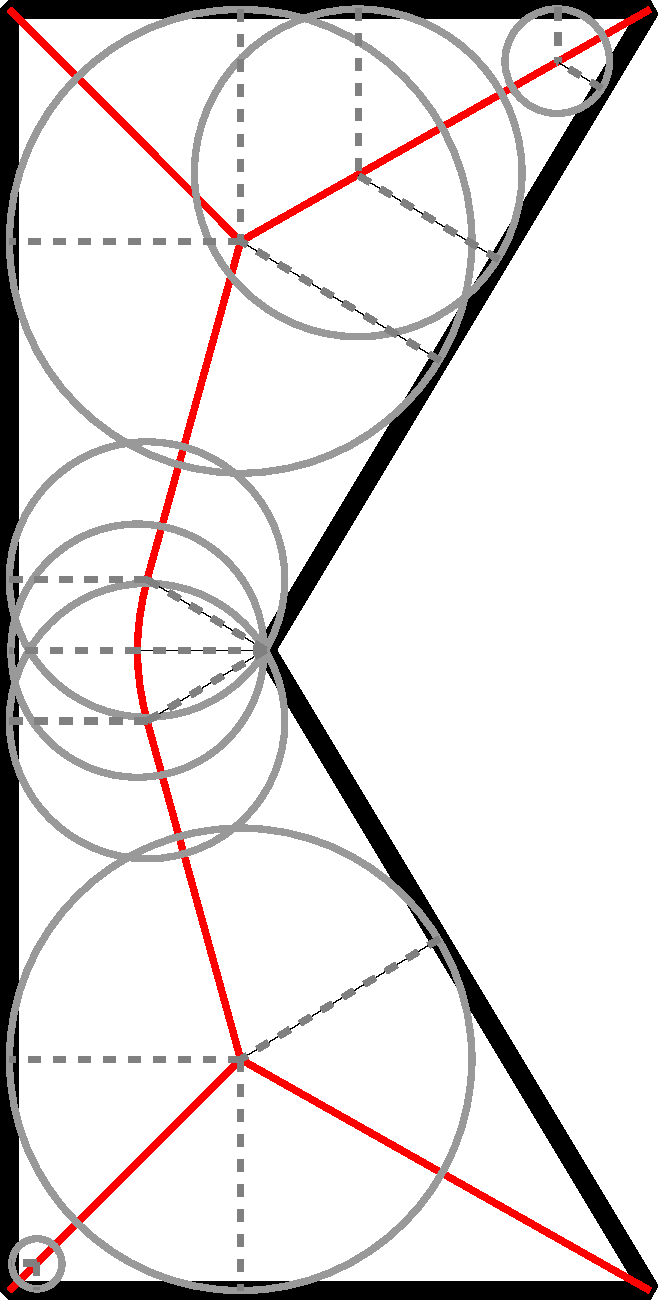
\includegraphics[height=1.5\columnwidth]{sources/method/MAT_explanation_circles.pdf}
\caption{Circles}
\label{MAT_explanation_circles}
\end{subfigure}
\begin{subfigure}{0.3\columnwidth}
\centering
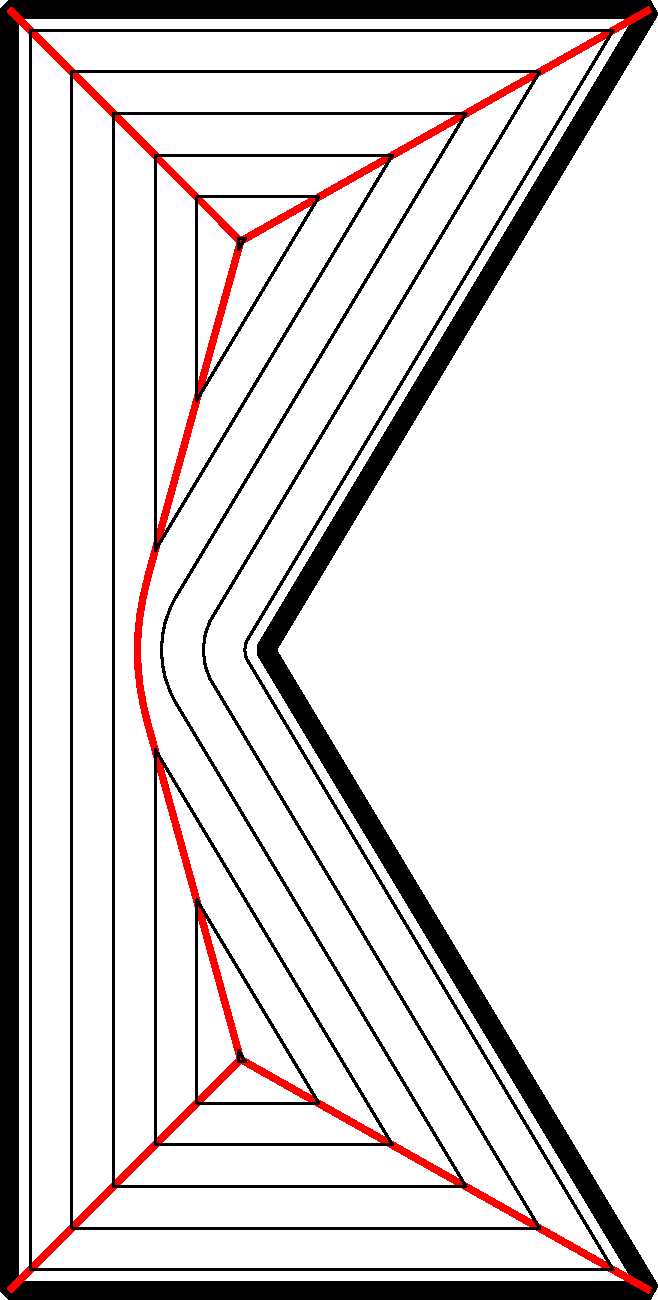
\includegraphics[height=1.5\columnwidth]{sources/method/MAT_explanation_wavefronts.pdf}
\caption{Wave-fronts}
\end{subfigure}
\begin{subfigure}{0.3\columnwidth}
\centering
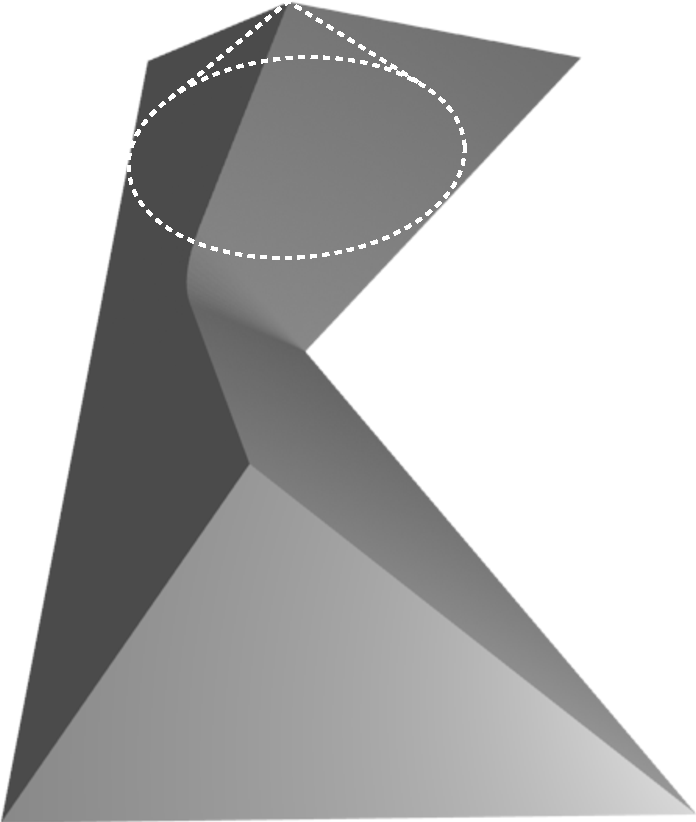
\includegraphics[height=1.5\columnwidth]{sources/method/MAT_explanation_cones.pdf}
\caption{Cones}
\end{subfigure}
\caption{
Medial axis representations.
The medial axis can be defined in terms of the the number of support points of the inscribed circles,
as the pinch sites in wave-fronts
or as ridges in a volume defined by the union of cones.
}
\label{MAT_explanation}
\end{figure}


\begin{figure}
\begin{subfigure}{0.3\columnwidth}
\centering
%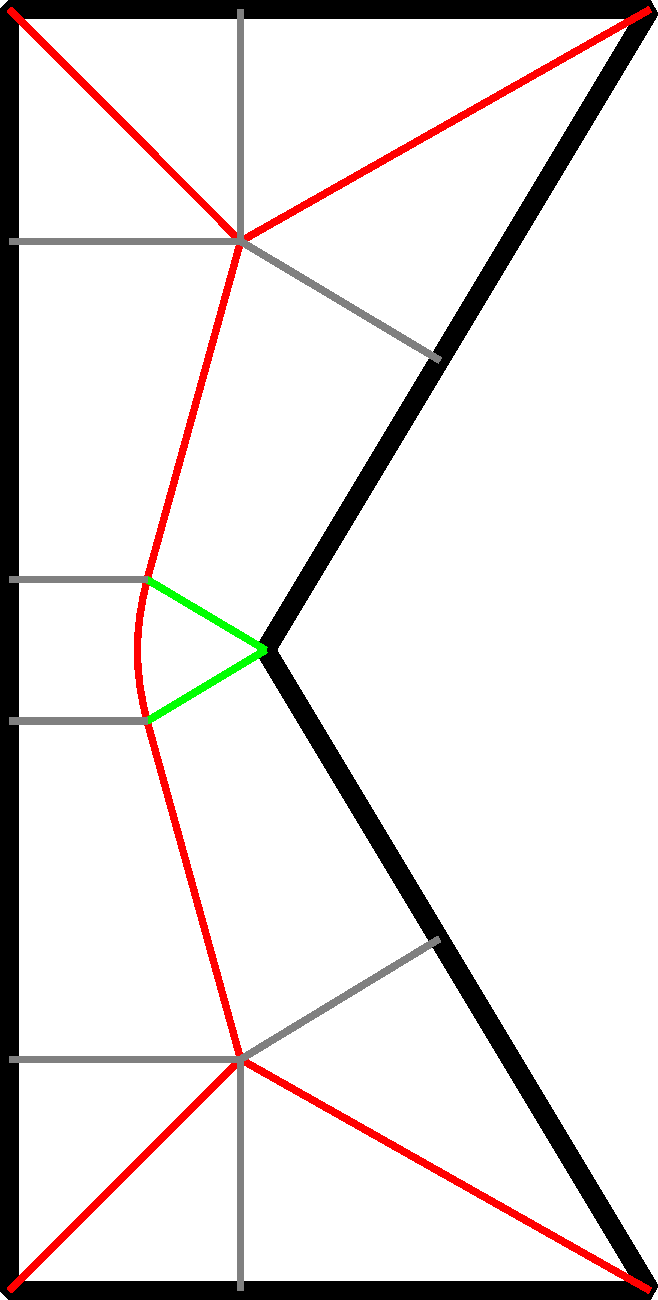
\includegraphics[height=1.5\columnwidth]{sources/method/MAT_explanation_shape_decomposition.pdf}
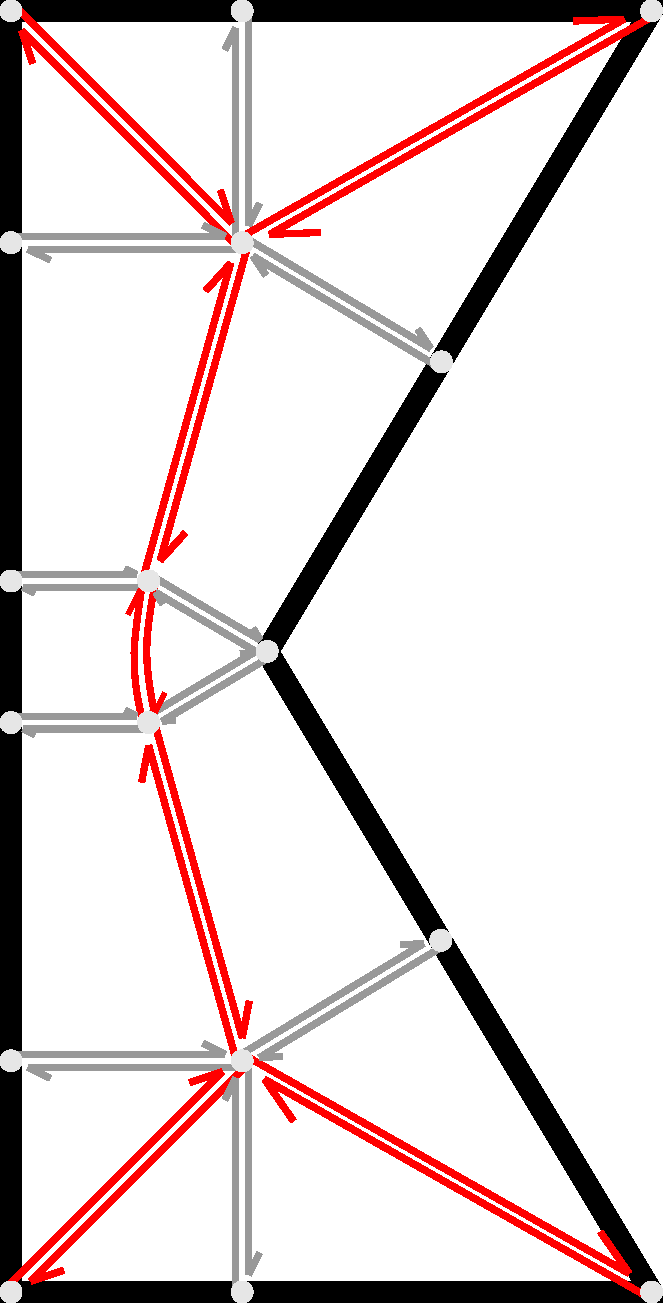
\includegraphics[height=1.5\columnwidth]{sources/method/half_edge_datastructure.pdf}
\caption{Simple case}
\label{shape_decomposition_simple}
\end{subfigure}
\begin{subfigure}{0.65\columnwidth}
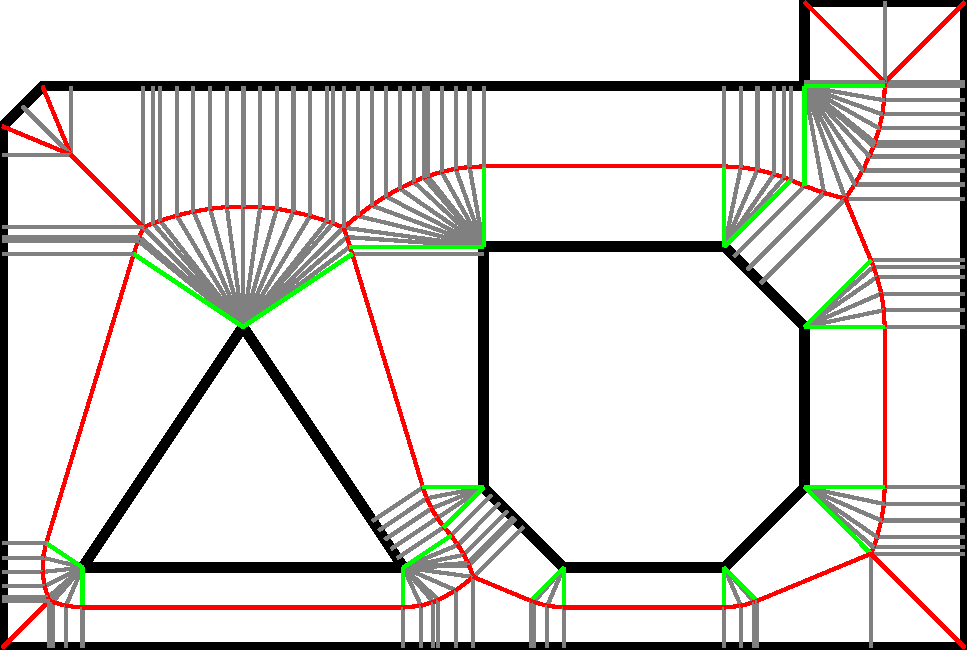
\includegraphics[width=\columnwidth]{sources/method/MAT_VD_VQ.pdf}
\caption{Complex case employing discretization}
\label{shape_decomp_complex}
\end{subfigure}
\caption{
Skeletonization of an outline shape (black).
Relation between the medial axis (red), the limited Voronoi Diagram (red and green) and the Skeletal Trapezoidation (red, green and gray): MAT $\subset$ Limited VD $\subset$ ST.
}
\label{skeletonization_comparison}
\end{figure}


\begin{figure} \centering
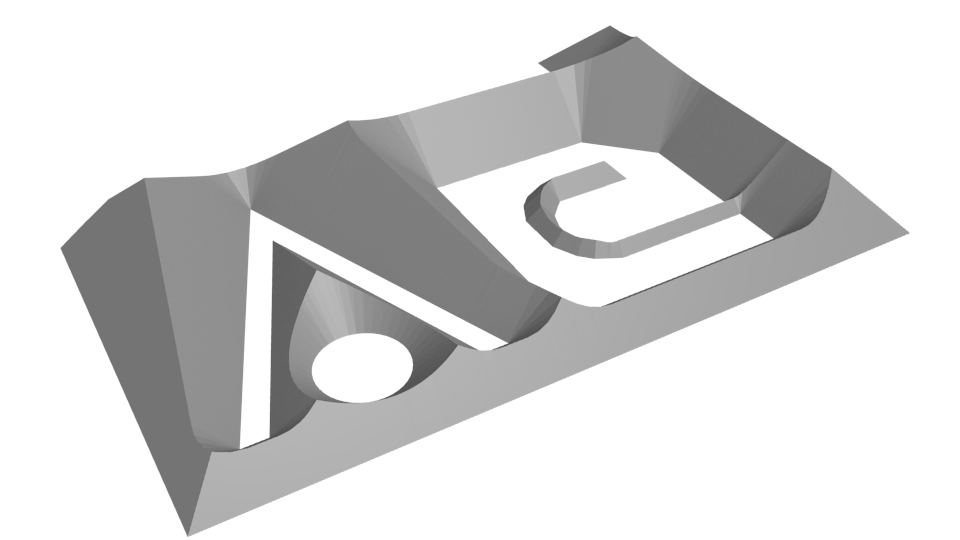
\includegraphics[width=.75\columnwidth]{sources/method/mat_3d_blender_render.png}
\caption{
Visualization of the distance field function as captured by the skeletal trapezoidation.
}
\label{mat_3d}
\end{figure}



\subsubsection{Skeletal trapezoidation}
We employ a shape decomposition proposed by \citeauthor{Ding2016a} which starts from the medial axis and further decomposes the outline shape into simple fragments. \cite{Ding2016a}
Each of the regions demarcated by the skeleton is further decomposed by adding radial bones from each node $v$ to its support $\text{sup}(v)$.
The resulting skeleton decomposes the outline shape into trapezoids and triangles.
We will therefore call this shape decomposition the \emph{Skeletal Trapezoidation} (ST).
(The concept of a trapezoidation conventionally allows for the degenerate case where a trapezoid resolves into a triangle. \cite{chazelle1984,fournier1984})
We represent such a skeleton in a standard half-edge data-structure.
See \cref{shape_decomposition_simple}.


The medial axis of a polygonal shape can be obtained from the Voronoi Diagram (VD) generated on the line segments and vertices of the shape, by throwing away all segments of the VD falling outside of the outline shape and throwing away the bones connected to concave vertices in the outline shape. \cite{lee1982medial}
However, the concave vertices are precisely in the support of the nodes to which those bones connect.
This means we can efficiently compute the ST from the VD by removing all segments which lie outside the outline shape and add radial bones to the nodes from there.
See \cref{skeletonization_comparison}.


We then also discretize parabolic segments and segments generated by two concave outline vertices into segments approximately as long as some constant $d^\text{discretization}$.
See \cref{discretization} and \cref{shape_decomp_complex}.
That way we can approximate the feature radius $R$ in between the two nodes $v_0$ and $v_1$ of a bone in the ST by interpolating linearly between $R(v_0)$ and $R(v_1)$.
This makes the skeleton capture a discrete approximation of the radius function which can then be used to create a triangulated 3D model of the conical representation of the medial axis; see \cref{mat_3d}.


\begin{figure}
\centering
%\begin{subfigure}{0.45\textwidth}
%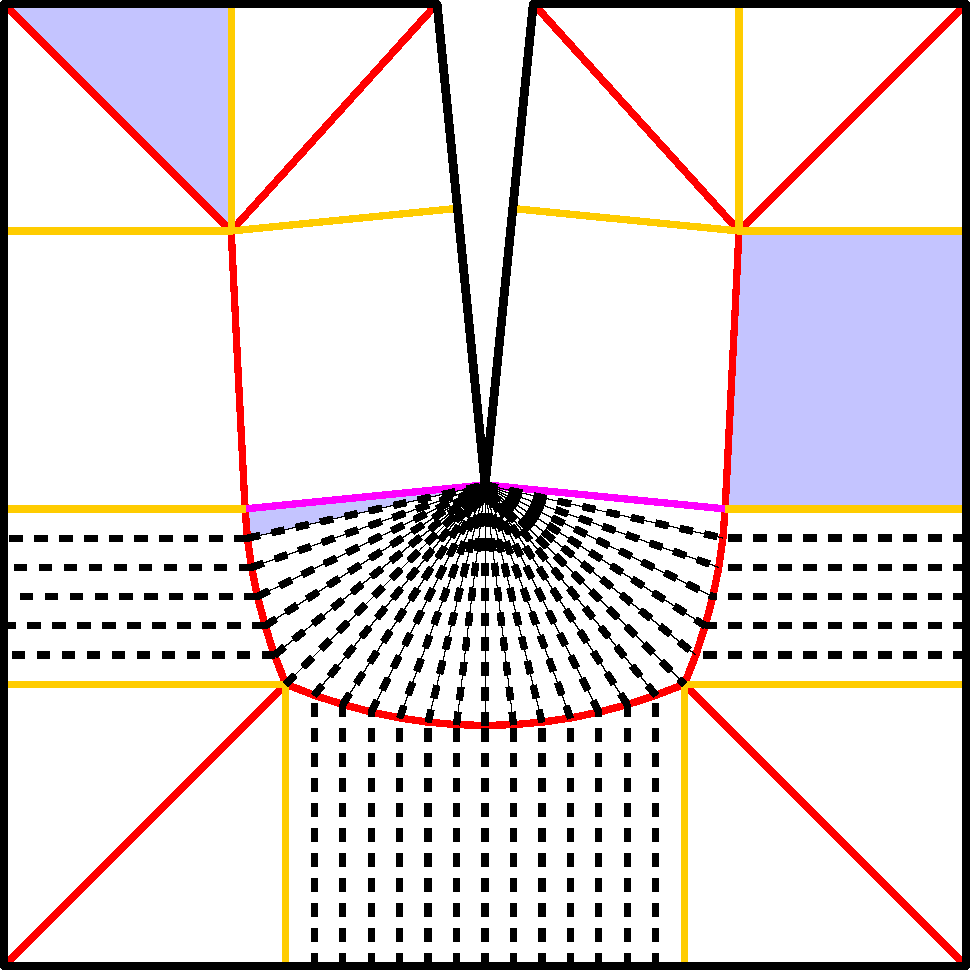
\includegraphics[width=\columnwidth]{sources/method/parabola_dip.pdf}
%\caption{asf}
%\end{subfigure}
%\begin{subfigure}{0.45\textwidth}
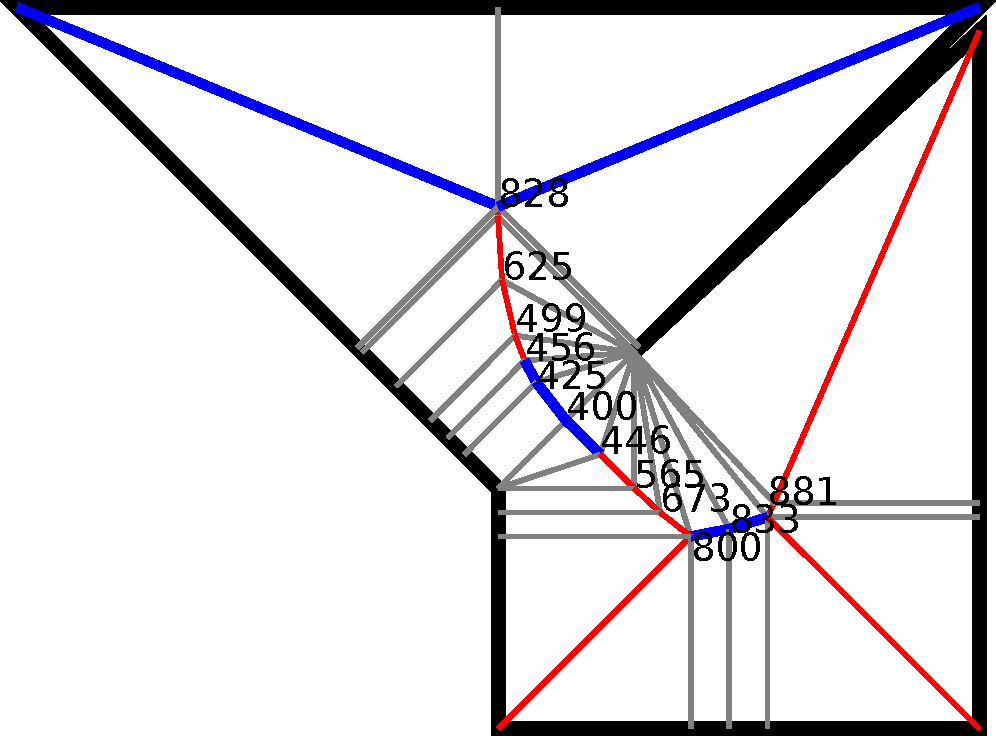
\includegraphics[width=\columnwidth]{sources/method/point-point_and_point-line_segments.pdf}
%\caption{Transitioning}
%\end{subfigure}
\caption{
Skeletal trapezoidation domain decomposition.
Medial axis (red and blue) is augmented with (gray) edges connecting each node to its nearest support points in the outline shape.
Parabolic medial axis segments are discretized and likewise for segments generated by two concave outline vertices, because the feature radius (black text in microns) doesn't increase linearly along those segments.
The blue segments are significant according to $\alpha_\text{max} = 135\degree$.
}
\label{discretization}
\end{figure}






\subsection{Bead counts}
We assign a bead count to each node in the skeleton which is in `the center' of the shape in a sense to be defined below.
Around regions where the bead count changes we introduce transition regions, so that we can smoothly change between regions with different bead count.

We mark a node of the skeleton as central if its feature radius is larger than that of all of the neighboring nodes in the skeletal graph.
We also mark whole bones as being central if they are significant according to a common significance measure.


\subsubsection{Significance measure}\label{sec:significance_measure}
Places where the naive concentric toolpathing strategy would create large underfill and overfill areas are locations which are in some sense \emph{central} to the shape.
This can be formalized by looking at the significance measure knows as the \emph{bisector angle}.
The bisector angle $\alpha$ is the angle $\angle{p_ovp_1}$ between a location $v$ on a bone of the skeleton and its two supporting polygon points $p_0$ and $p_1$.\cite{attali1996modeling}
Bones are significant if the bisector angle exceeds $\alpha_\text{max}$ which is governed by the beading strategy.

For a polygon with a pointy wedge area of an angle $\beta$, we have $\alpha = 180\degree - \beta$, which corresponds to overfill areas and underfill areas the size of $\nicefrac12 w^2 \left( \nicefrac14 \tan ( \alpha / 2) - \alpha / 2 \right)$ when filled using a naive strategy of constant bead width $w$.
See \cref{naive_overfill_underfill}.
The bisector angle is therefore an exact measure of the amount of overfill and underfill in the naive toolpaths of constant width.
%Contrary to related literature we will \emph{keep} the non-significant regions of the skeleton.
We mark all significant bones as such and contrary to related literature we keep the unmarked bones of the skeleton.
Our framework will decide on a beading at all of the marked nodes in `the center' nodes and apply the beading outward to the unmarked nodes.


\begin{figure}
\centering
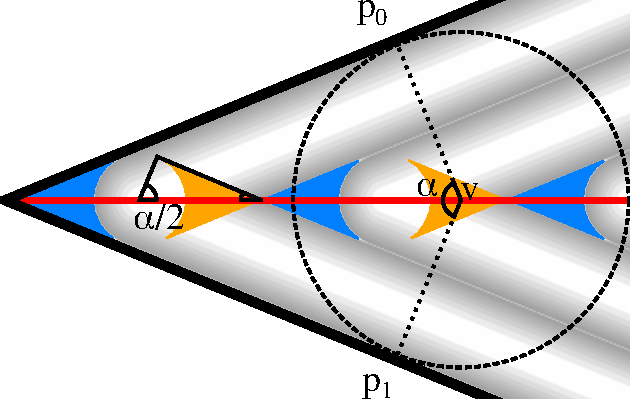
\includegraphics[width=\columnwidth]{sources/method/naive_overfill_underfill.pdf}
\caption{
Overfill and underfill areas in a naive beading using a constant bead width $w$ of a wedge area with vertex angle $\beta$.
The underfill areas (light blue) are mirrored versions of the overfill areas (dark red).
The bisector angle $a = 180\degree - \beta$ is the angle between a location $v$ and its support $p_0$ and $p_1$.
}
\label{naive_overfill_underfill}
\end{figure}


A computationally efficient way to compute $\alpha$ can be obtained by looking at the ratio between feature radius $R$ and the Euclidean distance:
if $ | R(v_1) - R(v_0) | / |v_1 - v_0| >  \cos(\alpha_\text{max} / 2)$ then $\alpha > \alpha_\text{max}$.
This means we can prevent executing trigonometric functions on \emph{each} of the bones in the skeleton.
See \cref{distance_based_angles}.
This ratio can readily be applied to simple skeleton segments to determine whether they are significant.
For skeletal segments generated by a polygon vertex at $(0,d)$ and a line segment through $(0,0)$ and $(0,\epsilon)$ or another vertex $(0,0)$, we can determine the significant portion by evaluating $\frac{\partial R}{\partial x} > \cos(\alpha_\text{max} / 2)$.
For parabolas we introduce extra points in the discretization at the two bounds where $| x | = d  / \tan(\alpha_\text{max} / 2)$
and for bones with vertex-vertex support we introduce discretization points at the two bounds where $| x | = \nicefrac12 d  / \tan(\alpha_\text{max} / 2)$.
This ensures that the discretization doesn't alter the extent and existence of significant regions.
See \cref{discretization}.


\begin{figure} \centering
\newlength{\significancePropertiesHeight}
\setlength{\significancePropertiesHeight}{.25\columnwidth}
\begin{subfigure}{0.35\columnwidth} \centering
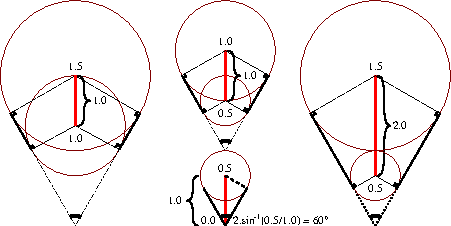
\includegraphics[height=\significancePropertiesHeight]{sources/method/distance_based_angles.pdf}
\caption{Significance}
\label{distance_based_angles}
\end{subfigure}
\begin{subfigure}{0.3\columnwidth} \centering
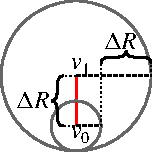
\includegraphics[height=\significancePropertiesHeight]{sources/method/distance_ratio_limit.pdf}
\caption{Distance}
\label{distance_ratio_limit}
\end{subfigure}
\begin{subfigure}{0.3\columnwidth} \centering
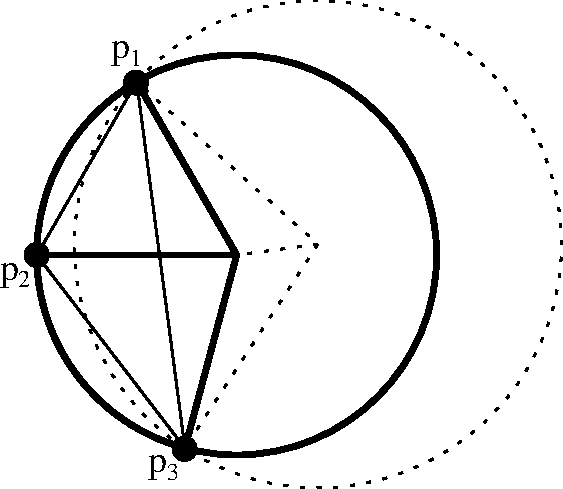
\includegraphics[height=\significancePropertiesHeight]{sources/method/branch_upward_edge_property.pdf}
\caption{Upward edge}
\label{branch_upward_edge_property}
\end{subfigure}
\caption{
Properties of feature radius $R$.
Part of outline shape in thick black,
skeleton in red,
inscribed circle in gray,
radii in dashed lines.
\subref{distance_based_angles} The significance measure can be simplified using $\alpha = 2 \gamma = 2 \cos^{-1} \Delta R / |v_1 - v_0|$.
\subref{distance_ratio_limit} The distance $|v_1 - v_0| > \Delta R$ because otherwise the feature radius would not be one of an inscribed circle.
\subref{branch_upward_edge_property} The radial distance can only increase along one edge around a branch point in the medial axis.
}
\end{figure}


\subsubsection{Properties of significant regions}
%\begin{lemma} \label{min_euclidean_distance} >> this paragraph contains two lemmas and a concluding remark!
The Euclidean distance between two skeletal vertices can never be less than the difference in the feature radius $R$ measure between the vertices.
See \cref{distance_ratio_limit}.
The condition $|v - p| = \Delta R$ is true exactly for those sekeletal bones between a node $v$ and an outline location $p$ added by the trapezoidation, which means that the trapezoidation never introduces marked bones, so we can perform the trapezoidation after marking.


\iffalse
% This fact is not used anymore, because we change the marking such that it doesn't hold for marked edges any more.
A node in the graph can have at most two significant edges.
For a node in the VD $v$ with a support of three points on the outline polygon $p_1, p_2, p_3$, the bisector angles $\angle{p_1vp_2} + \angle{p_2vp_3} + \angle{p_3vp_1} = 360\degree$, so if two angles are more than $\alpha_\text{max} > 120\degree$ the third one needs to be smaller than $360\degree - 2\alpha_\text{max} < 120\degree$ and therefore nonsignificant.
% However, because of some filtering operations this property does not neccesarily hold for the markings.
The extra edges added to the VD to form the ST can never be significant because their bisector angle is \SI{0}{\degree} by definition,
so the nodes of the ST also have at most two significant edges.
\fi

\begin{lemma}\label{saddle_points_are_marked}
A saddle point is always marked, i.e.\
when traversing the skeletal graph from one locally maximal $R$ to another we must pass through a significant region.
\end{lemma}
\begin{proof}
You will either go through the marked region of a discretized parabola or of a segment with two polygonal vertices as support.
This means that the feature radius function in between marked regions is always monotonic.
This means that when propagating beadings downward from marked regions they can never conflict in the middle - they will always conflict at either marked region.
\end{proof}

\begin{lemma}\label{single_upward_edge}
From any node in the graph which is not a saddle point there is at most a single edge going upward.
\end{lemma}
\begin{proof}
Any branch point $v$ in the MAT coincides with the circumcircle of its support $p_0, p_1, p_2$.
If $v$ lies within $\triangle p_0 p_1 p_2$ it is a local maximum and otherwise we will show it has exactly one upward edge.
If $v$ lies outside of $\triangle p_0 p_1 p_2$ then those support points lie within a \SI{180}{\degree} range from $v$
and one point lies in the middle, say $\angle p_0 + \angle p_1 = \angle p_2$.
Then a circle with radius $R(v) + \epsilon$ around $v'$ such that $|v-v'| < \epsilon$ can only touch $p_0$ and $p_2$.
See \cref{branch_upward_edge_property}.
%See VoronoiQuadrangulation::filterUnmarkedRegions
Bones added because of the trapezoidation always go down to $R=0$, so these don't change the property that each node has at most a single upward edge.
This means that walking up the graph from a marked region to a local maximum follows a single path without branching.
\end{proof}




\iffalse
% This fact is not used anymore, because we change the marking such that it doesn't hold for marked edges any more.
The two downward edges from a branch point cannot both be significant.
A branch point which is not a local maximum generated by the support points $p_1, p_2, p_3$ has bisector angles such that $\triangle p_1 p_2 p_3$ has its circumcentre $v$ outside of the triangle, because otherwise the feature radius decreases in all directions.
This means that all support points lie within a \SI{180}{\degree} range around the node. 
Suppose the one edge going upward is generated by $p_1$ and $p_3$.
Then the bisector angle $\angle p_1 v p_3 < 180\degree$ and $\angle p_1 v p_2 + \angle p_2 v p_3 < 180\degree$,
so if $\angle p_1 v p_2 < 120\degree$ then $\angle p_2 v p_3 < 60\degree$ and is therefore not significant. 
%so at most either of $\angle p_1 v p_2$ and $\angle p_2 v p_3$ has a significant bisector angle.
\fi



\subsubsection{Marking filtering}
Using the significance measure and the local maximum feature radius condition we initialize all marked bones and nodes.
We then filter out high frequency changes in the marking in order to ensure smooth output toolpaths. 
We perform filtering on the unmarked regions, so that the properties of significant regions mentioned above remain valid.
From each marked node $v_0$ with an upward unmarked bone attached we walk along the upward edges (which cannot branch because of \cref{single_upward_edge}).
If the total length traversed until we reach another marked node $v_1$ is shorter than some filter distance $d_\text{max}^\text{unmarked}$, we mark all bones encountered as being central.





\subsubsection{Initial bead count}
In order to apply a beading strategy to the ST we first assign bead counts to the central regions and then decide on how to apply those bead counts outward.
In order to decide on an initial bead count, we require a function mapping a feature diameter to a bead count: $b: \mathbb{R} \to \mathbb{N}$.
(The feature diameter is twice the radius.)
For example we might choose to round to the nearest integer multiple of some preferred width $w_\text{pref}$: $b(d) = \left\lfloor \nicefrac{d}{w_\text{pref}} + \nicefrac12 \right\rfloor$.
The function $b$ is determined by the beading strategy and is required to increase monotonically with the input feature diameter.

We first assign each marked node $v$ of the skeleton an initial bead count $b^*_v \leftarrow b(2R(v))$, but it is modified in order to prevent high frequency changes in bead count and it is changed in order to account for smooth transitions in bead count.
See \cref{beading_transitioning_filtering__bead_count}.

We also filter unmarked regions where the bead count remains constant in order to limit the extent of a problem handled in \cref{section_beading_conflicts}.
From each marked node $v_0$ with an upward unmarked bone attached we walk along the upward edges (which cannot branch because of \cref{single_upward_edge}) until we hit another marked node $v_1$.
If the upper node has the same bead count $b^*_{v_1} = b^*_{v_0}$ we mark all bones and nodes $v$ in between, and set the bead count $b^*_v \leftarrow b^*_{v_0}$.


\begin{figure*}
\centering
\setlength{\figwidth}{0.15\textwidth}
\begin{subfigure}{\figwidth}
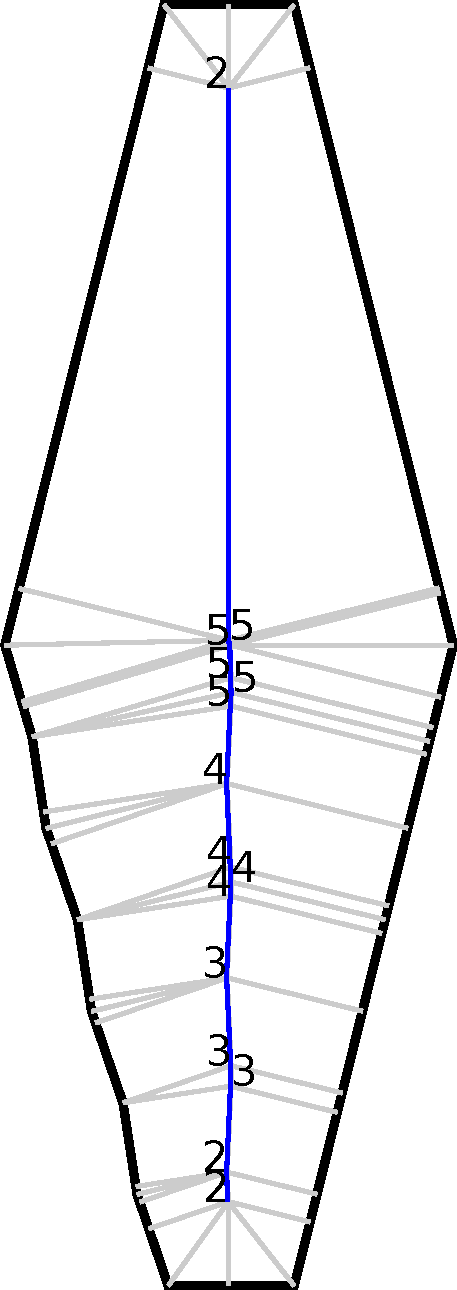
\includegraphics[width=\columnwidth]{sources/method/beading_transitioning_filtering__bead_count.pdf}
\caption{Initial bead counts}\label{beading_transitioning_filtering__bead_count}
\end{subfigure}
\begin{subfigure}{\figwidth}
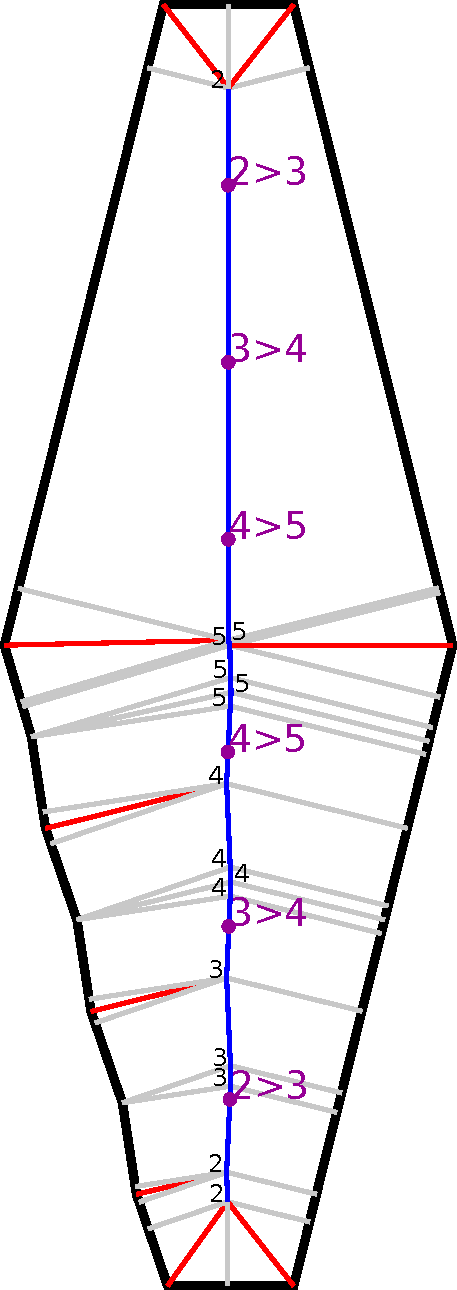
\includegraphics[width=\columnwidth]{sources/method/beading_transitioning_filtering__transition_mids.pdf}
\caption{Transition anchors}\label{beading_transitioning_filtering__transition_mids}
\end{subfigure}
\begin{subfigure}{\figwidth}
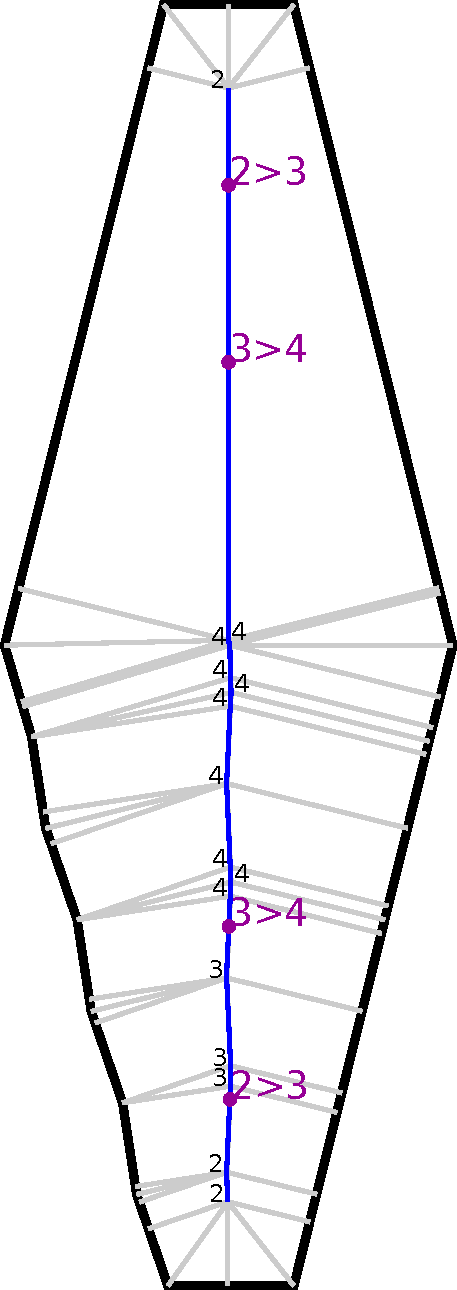
\includegraphics[width=\columnwidth]{sources/method/beading_transitioning_filtering__filtered.pdf}
\caption{Filtered anchors}\label{beading_transitioning_filtering__filtered}
\end{subfigure}
\begin{subfigure}{\figwidth}
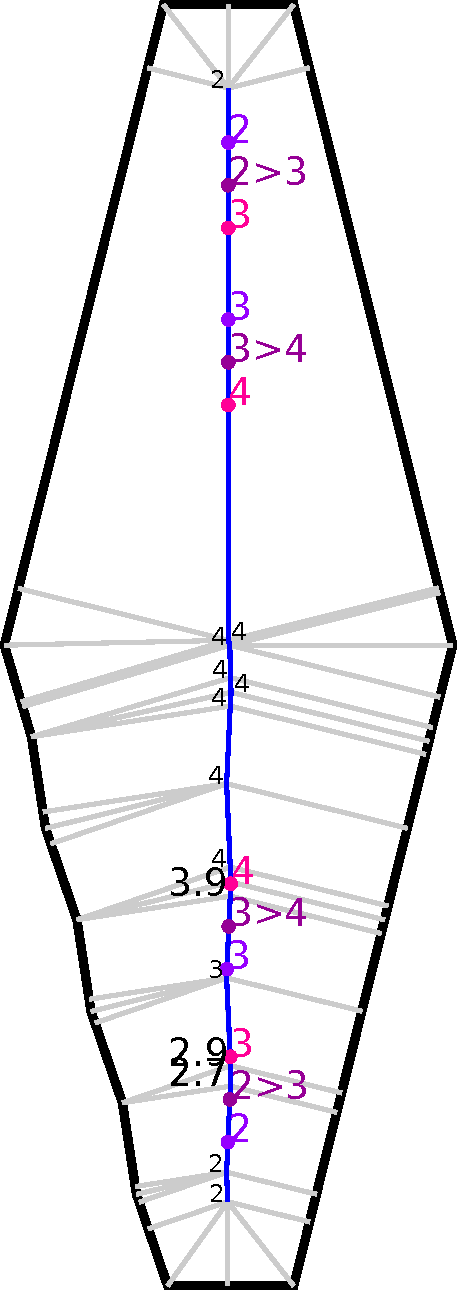
\includegraphics[width=\columnwidth]{sources/method/beading_transitioning_filtering__transition_ends.pdf}
\caption{Transition ends}\label{beading_transitioning_filtering__transition_ends}
\end{subfigure}
\begin{subfigure}{\figwidth}
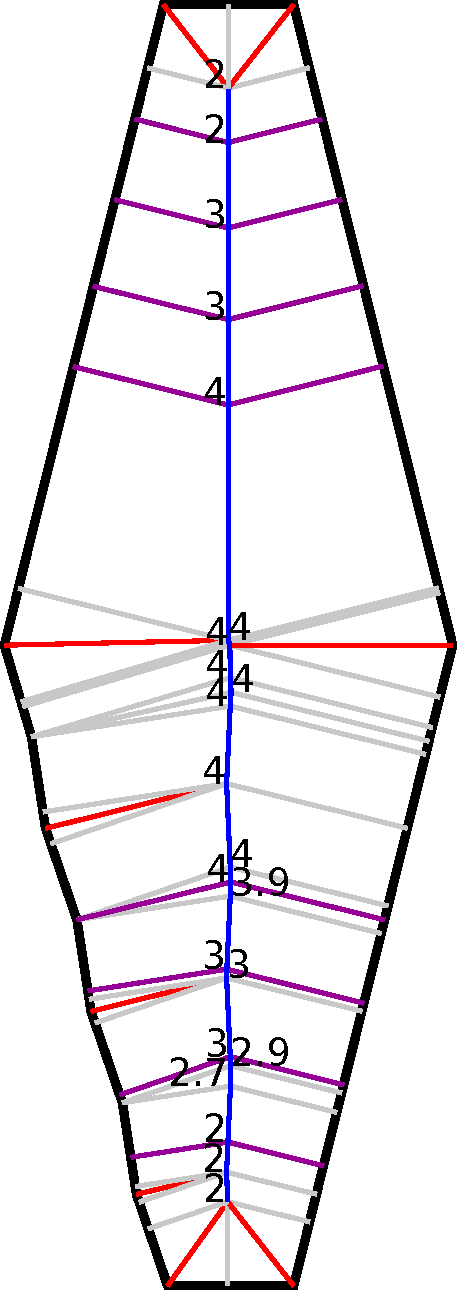
\includegraphics[width=\columnwidth]{sources/method/beading_transitioning_filtering__transitions_applied.pdf}
\caption{Radial bones}\label{beading_transitioning_filtering__transitions_applied}
\end{subfigure}
\caption{
Applying bead counts and transitioning on a shape showing the difference between a simple skeleton (top) and a mirrored version with small perturbations in the outline (bottom).
Outline in black, medial axis edges in red, radial edges in grey.
\subref{beading_transitioning_filtering__bead_count} First we initialize the bead counts (black) in the marked regions (blue).
\subref{beading_transitioning_filtering__transition_mids} We then extract the anchor locations (purple) of the transitions to a different bead count should be.
\subref{beading_transitioning_filtering__filtered}We then filter out regions of constant bead count.
\subref{beading_transitioning_filtering__transition_ends} We then calculate the end locations (magenta, pink) of the transitions and modify the bead count at nodes in between to fractional values.
\subref{beading_transitioning_filtering__transitions_applied} Finally we introduce nodes at the ends and introduce radial edges (purple) as per the trapezoidation constraint.
The symmetry in the result shows that transitioning is robust against small perturbations in the outline shape.
}
\label{beading_transitioning_filtering}
\end{figure*}


\subsubsection{Transitioning}
In order to prevent discontinuities in the toolpaths around locations where the bead count changes, we need a way to smoothly transition to a different number of beads around locations where the 3D model has a changing radius.
See \cref{transitions}.
The length along the marked region of a transition from bead count $n$ to $n+1$ is determined by some function $t(n)$.
Because transitions in bead count only occurs in locations where the preferred bead count $b$ changes, we introduce $b^{-1}(n) := \argmax_d b(d) = n$.

For each marked bone between $v_0$ and $v_1$ with $b^*_{v_0} \neq b^*_{v_1}$ we introduce transitions.
A transition from bead count $n$ to $n+1$ will be placed anchored on each location $v_x$ where $R(v_x) = b^{-1}(n)$.
We can compute the location of the anchor simply as
$$v_x = v_0 + (v_1 - v_0) \frac{ b^{-1}(n) - R(v_0) }{ R(v_1) - R(v_0) }$$
for each $n$ such that $b^*_{v_0}<n<b^*_{v_1}$.
See \cref{beading_transitioning_filtering__transition_mids}.

A transition with length $t(n)$ will be placed somewhere covering the anchor position.
We require an additional function to be specified by the beading strategy: $t_0(n)$ determines the distance between the lower end of a transition from bead count $n$ to $n+1$ and the anchor point - as measured along the marked bones of the skeleton.
From that we calculate $t_1(n) = t(n) - t_0(n)$ for the distance from the anchor to the upper end of the transition.
The transitions lengths should be such that they fit between anchor locations of two consecutive transitions even for a bone with high bisector angle:
$$t_1(n) + t_0(n+1) < \frac{ b^{-1}(n + 1) - b^{-1}(n) }{ \cos \nicefrac12 \alpha_\text{max}}$$
for each $n \in \mathbb{N}$.
See \cref{transition_placement}.



\begin{figure}
\centering
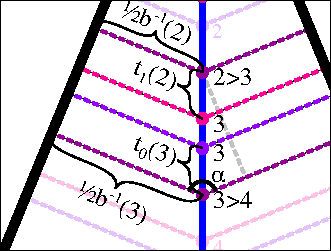
\includegraphics[width=.4\columnwidth]{sources/method/transition_length_limit.pdf}
\caption{
Placement of transition ends (magenta and pink) with respect to the anchor positions of the transitions (purple) on a skeleton segment (blue) with bisector angle $\alpha \approx \SI{135}{\degree}$.
The distance between the anchor position and the upper end ($t_1$) and the distance between the anchor position and the lower end of the transition ($t_0$) should add up to less than the total distance between the anchor positions, which is limited by $\alpha_\text{max}$.
}
\label{transition_placement}
\end{figure}


In order to prevent frequent oscillations in the bead count, we filter locally maximal or minimal bead count regions.
For each edge which contains a transition anchor we walk along the marked regions until we encounter another anchor.
If the other anchor is a transition in the opposite direction and the traversed distance is within some limit $d_\text{max}^\text{transition}$ we remove the transitions and set the bead counts at all nodes in the filtered region to the surrounding bead counts.
If we hit the end of a marked region and the traversed distance from the anchor point is less than the distance $t_{0}(n)$ or $t_{1}(n)$ to the transition end we dissolve the bead count region in the same manner.
See \cref{beading_transitioning_filtering__filtered}.

In order to generate the lower and upper end point of the transitions we walk downward and upward along the marked regions from each anchor position $v$ until we have traversed the corresponding distance of $t_{0}(n)$ or $t_{1}(n)$.
If there is any node $v_x$ in between $v$ and $v_0$ or $v_1$ we assign it a fractional bead count by linear interpolation: $b^*_{v_x} = n + D(v_0, v_x)/t(n)$, where $D(.)$ is the cumulative distance measured along the marked bone(s).
See \cref{beading_transitioning_filtering__transition_ends}.
These fractional bead counts will be used in \cref{section_beading_interpolation}.

Finally we perform the graph update by introducing nodes at the transition ends and introducing radial bones from these new nodes to the outline as per the trapezoidation requirement.
See \cref{beading_transitioning_filtering__transitions_applied}.


\begin{figure}
\centering
\setlength{\figwidth}{\columnwidth}
\begin{subfigure}{0.9\figwidth}
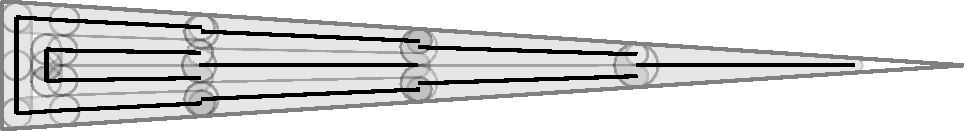
\includegraphics[width=\columnwidth]{sources/method/wedge_distributed_generated__no_transitions.pdf}
\caption{Without transitioning}
\end{subfigure}
\begin{subfigure}{0.9\figwidth}
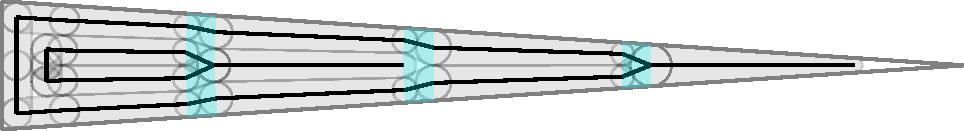
\includegraphics[width=\columnwidth]{sources/method/wedge_distributed_generated.pdf}
\caption{Transitioning}
\end{subfigure}
\caption{
Discontinuities around regions where the bead count changes are prevented by transition regions (highlighted in cyan).
}
\label{transitions}
\end{figure}







\subsection{Toolpath extraction}
\label{section_toolpath_extraction}
Now that we have decided on the bead counts in the central marked regions, we can apply those bead counts outward along the unmarked bones of the skeleton in order to define the locations of the toolpath junctions.
Because there is a plethora ways to cover a distance $d$ with $n$ beads, the placement of junctions depends on the chosen beading strategy.
The beading strategy is used to generate the bead widths and radial distances at which the junctions are placed for each node: the \emph{beading}.
That beading information is then propagated along the unmarked bones of the skeleton, so that we can generate the junctions on each unmarked bone.
The junctions are then connected together per trapezoid in order to form the final toolpaths.


\begin{definition}\label{beading_strategy_definition}
We define a beading strategy as the following set:
$$
\left\{ \alpha_\text{max}, b(d), t(n), t_0(n), W(n, d), L(n, d) \right\}
$$
where
$\alpha_{\text{max}}$ (the limit bisector angle),
$b(d)$ (optimal bead count),
$t(n)$ (transition length)
and
$t_0(n)$ (transition anchor position) have already been defined above.
We introduce here
$W(n, d)$, which gives the sequence of bead widths to cover a distance $d$ using $n$ beads
and
$L(n, d)$, which gives the sequence of toolpath positions as radial distances from the outline to cover a distance $d$ using $n$ beads.
\end{definition}


The following restrictions hold:
\begin{enumerate}
\item $W$ is symmetric: $W(n, d)_i = W(n, d)_{n-i-1}$
\item $L$ is symmetric in $d$: $L(n, d)_i = d - L(n, d)_{n-i-1}$
\item $W_n$ is monotonic and continuous at each bead index $n$ for constant bead count $c$: $0 \leq \frac{\partial W(c, d)_n}{\partial d} < \infty$.
\end{enumerate}


\begin{definition}
By applying the beading strategy to a skeleton location $v$ and a predetermined bead count $n$ we get a beading $B$, which is defined as the following set:
$$
\left\{ d, n, w_i, l_i  \right\}
$$
where
$d = 2 R(v)$ is the diameter associated with $v$,
$n$ is the bead count,
$w_i$ is the bead width of the bead with index $0 \leq i < n$ counting from the outline inward
and
$l_i$ is the distance of the toolpath location of bead with index $0 \leq i < n$.
\end{definition}



\subsubsection{Beading interpolation}\label{section_beading_interpolation}
Skeletal nodes which are in the middle of a transition have obtained a fractional bead count, but the functions defined in the beading strategy are only defined on natural numbers.
The fractional part of the bead count is used to interpolate between two beadings defined on the fractional bead count rounded up and down.
Suppose we want to interpolate between two beadings $B^V$ and $B^W$, for which $n^{B^V} < n^{B^W}$.
We interpolate the diameter $d$, widths $w_i$ and locations $l_i$ for indices $i < \frac12 n^{B^V}$ linearly and enforce the symmetry constraints on the upper indices.
See \cref{beading_interpolation}.
The linear interpolation enforces robustness against small perturbations in the outline shape which cause extra bones to appear in the skeleton inside of transition regions.

\iffalse
In order to create an interpolated beading $B = xB^V + (1-x) B^W$, for some $0<x<1$
we calculate:
\begin{align*}
n^{B} &= n^{B^W} \\
d^B &= x d^{B^V} + (1-x) d^{B^W} \\
w_i^{B} &= w_{n^B-i}^{B} = x w_i^{B^V} + (1-x) w_i^{B^W} \text{ for } i < \frac12 n^{B^V} \\
%  w_{frac{n}{2}^B - frac12}  = something difficult \text{ if } n \mod 2 == 1
w_i^{B} &= w_i^{B^W} \text{ otherwise}\\
l_i^{B} &= 
\begin{cases} 
x l_i^{B^V} + (1-x) l_i^{B^W} & \text{ for } i < \frac12 (n^{B^V} - 1) \\
d^B - x l_{i-n^{B^W}+n^{B^V}}^{B^V} + (1-x) l_i^{B^W} & \text{ for } i > n^B - 1 - \frac12 (n^{B^V} - 1) \\
\frac12 d^B  & \text{ if $n^B$ is odd and } i = (n^B - 1) / 2 \\
l_i^{B^W} - l_{n^{B^V}-1}^{B^W} + l_{n^{B^V}-1}^B & \text{ otherwise}
\end{cases}
\end{align*}
\fi

\begin{figure}
\centering
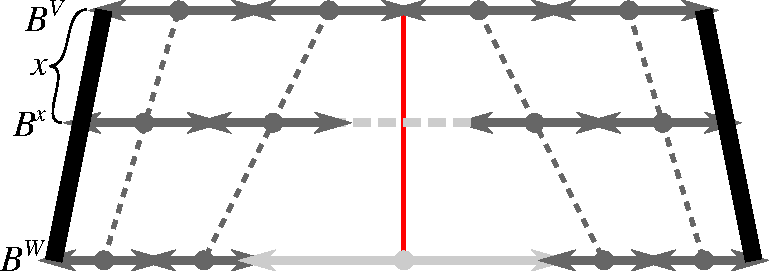
\includegraphics[width=.8\columnwidth]{sources/method/beading_interpolation_v2.pdf}
\caption{
Interpolation between two beadings $B^V$ and $B^W$ with a ratio $x$ results in a beading $B^x$.
Distances between the thick black lines constitute diameters $d$,
the toolpath locations are visualized as dots,
the widths are visualized as bidirection arrows
and the middle is highlighted in red.
}
\label{beading_interpolation}
\end{figure}


\subsubsection{Beading propagation}\label{section_beading_conflicts}
Because the beading information will be propagated outward from the central marked regions, beading conflicts can arise where a marked bone has unmarked upward edges attached to them, since beading will also be propagated down from the local maxima or other higher marked regions.
See \cref{beading_conflict_problem}.
In such a case we will interpolate between the lower beading and the beading propagated from above,
starting from the lower marked node and ending at a distance $t_\text{beading}$ upward.
At the nodes in between we will apply the interpolation between the two beadings and propagate the interpolated beading outward from those nodes.
This interpolation is performed during the beading propagation algorithm.
\todo{Make a better figure for this.}


\begin{figure}
\centering
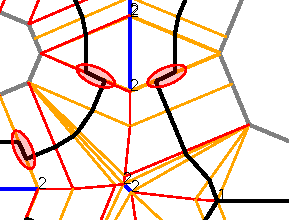
\includegraphics[width=.5\columnwidth]{sources/method/transition_to_insignificance_problem.pdf}
\caption{
Problems at the boundary of marked regions highlighted with red ovals.
The beading approach from the marked region (blue) results in toolpaths (black) which don't line up with the approach following from the beading which results from the bead count at the local maximum in the bottom center.
}
\label{beading_conflict_problem}
\end{figure}

After each marked node is assigned a beading by the beading strategy, we propagate the beadings outward to all nodes in the ST.
The beading propagation is performed in two stages: an upward stage and a downward phases.
%First we sort all upward half-edges on the radial distance of their destination node, so that we can efficiently flood fill the beading information.
In the upward phase we walk from each marked node upward along unmarked edges and map each node encountered to a pair consisting of the traversed distance and the bottom source beading.
In the downward phase we walk from each marked node downward along unmarked edges and map each node to a pair consisting of the traversed distance and the upper source beading -
however, if we encounter a node which was already mapped to an upward propagated beading we employ the interpolation scheme described above in order to define the beading, which is then further propagated downward.
This is implemented in a flood-fill fashion: see \cref{alg_beading_propagation}.

\begin{algorithm}
\caption{Beading propagation}
\label{alg_beading_propagation}
\begin{algorithmic}
\ForAll{$v \in$ nodes}
	\If {marked($v$)} $\text{map}[v] = (0, B(b^*_v, 2 R(v)))$ \EndIf
\EndFor
\ForAll{$e \in$ edges}
	\If {$R(v_0^e) < R(v_1^e)$}
		% \State 
		upwardEdges.add($e$)
	\EndIf
\EndFor
\State upwardEdges.sort($\uplambda e_1 e_2 . R(v_1^{e_1}) < R(v_1^{e_2})$) \Comment {low to high $v_1$}
\ForAll{$e \in$ upwardEdges} \Comment{upward phase}
	\If {$\text{map}[v_0^e] \land \neg \text{map}[v_1^e$]}
    		\State $(d, B) = \text{map}[v_0^e]$
    		\State $\text{map}[v_1^e] \leftarrow (d + |v_1^e - v_0^e|, B)$
	\EndIf
\EndFor
\ForAll{$e \in$ reverse(upwardEdges)} \Comment{downward phase}
	\If {$\text{map}[v_1^e]$}
    		\State $(d, B) \leftarrow \text{map}[v_1^e]$
    		% d + |v_1^e - v_0^e|
    		\If {$\text{map}[v_0^e]$}
    			\State $(d_0, B_0) = \text{map}[v_0^e]$
    			\State $B \leftarrow \text{interpolate}(\min(1, d_0 /  t_\text{beading}), B_0, B)$
    		\EndIf
    		\State $\text{map}[v_1^e] \leftarrow (0, B)$
	\EndIf
\EndFor
\end{algorithmic}
\end{algorithm}




\subsubsection{Toolpath extraction algorithm}
Now that each node has a beading associated with it we can apply the beading to generate the junctions of the toolpaths.
For each upward half-edge $e$ we generate each junction $J$ based on the beading $B = B^{v_1^e}$:
\begin{align*}
J &= \{ v, w, i \} \\ 
v &= v_1^e + (v_0^e - v_1^e) \frac{R(v_1^e) - l_i^B}{R(v_1^e) - R(v_0^e)} \\ 
w &= w_i^B
% \\ i^J &= i
\end{align*}
for any $i$ for which $R(v_0^e) < l_i^B \leq R(v_1^e)$.
See \cref{junction_placement}.
We store all junctions of a segment in a mapping from edge to a list of junctions.


\begin{figure}
\centering
\setlength{\figheight}{.29\columnwidth}
\begin{subfigure}{0.14\columnwidth}\centering
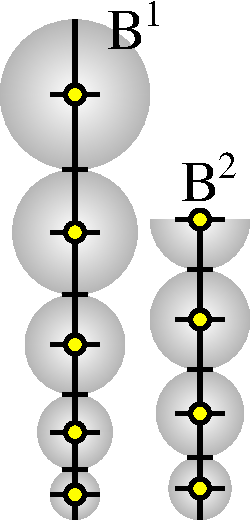
\includegraphics[height=\figheight]{sources/method/trapezoid_beading_beading.pdf}
\caption{Beadings}\label{trapezoid_beading_beading}
\end{subfigure}
\begin{subfigure}{0.5\columnwidth}\centering
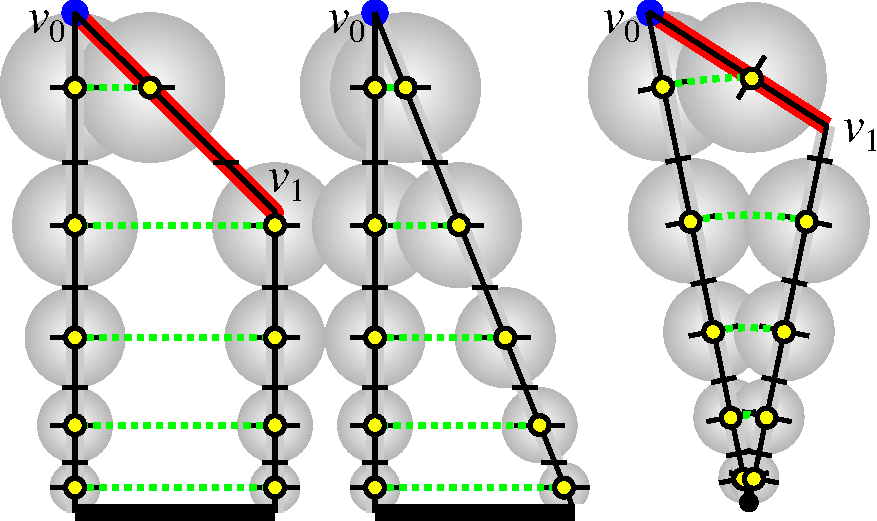
\includegraphics[height=\figheight]{sources/method/trapezoid_beading_propagated.pdf}
\caption{Single beading propagated to all nodes}\label{trapezoid_beading_propagated}
\end{subfigure}
\begin{subfigure}{0.34\columnwidth}\centering
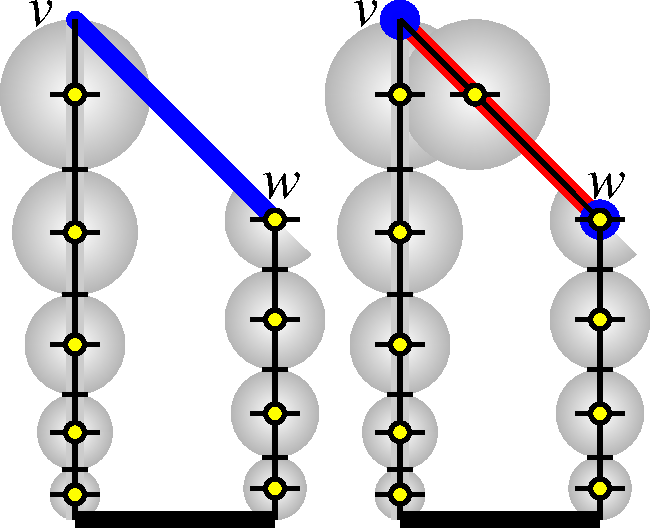
\includegraphics[height=\figheight]{sources/method/trapezoid_beading_separate.pdf}
\caption{Separate beadings at either top node}\label{trapezoid_beading_separate}
\end{subfigure}
\caption{
Applying beadings togenerate junctions along trapezoids.
\subref{trapezoid_beading_beading} shows half of the locations $L(n,d)_i$ and widths $W(n,d)_i$ of two arbitrary different beadings.
\subref{trapezoid_beading_propagated} shows the application of $B^1$ to the various types of trapezoid.
\subref{trapezoid_beading_separate} shows how a trapezoid with a marked edge will have two different beadings assigned, which will generate their respective junctions along the support bones.
No junctions will be generated along marked bones.
Wide black lines are outline segments, marked nodes and bones in blue, the junctions in yellow and green wavefronts of equidistant radial distance at $R = L(n,d)_i$.
}
\label{junction_placement}
\end{figure}


We then generate bead segments for each trapezoid by connecting together the junctions of the same index.
See \cref{segment_generation}.
If the amount of junctions on both sides of the trapezoid is not the same then this trapezoid is in a transition and we leave one inner junction unconnected.
If a central edge has both nodes with an odd bead count assigned to it $b^* \bmod 2 = 1 $ we should prevent the algorithm from generating the center segment from both trapezoids.
We therefore use some arbitrary condition to decide which one of the two to include based on the ordering of the coordinates of $v_0$ and $v_1$.

Each of the trapezoids is connecting to a single outline polygon.
By traversing the trapezoids in the domain of each outline polygon in order we can efficiently connect all segments into polylines.
See \cref{segment_generation}.
In a final step we connect the ends of polylines together, so that the final toolpaths contain both polygons and polylines.

\begin{figure}
\centering
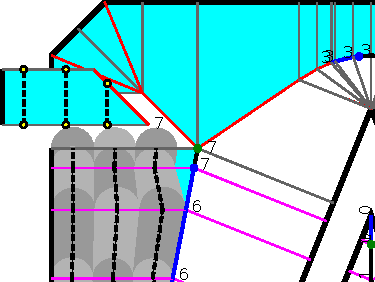
\includegraphics[width=.5\columnwidth]{sources/method/segment_generation.pdf}
\caption{
Generating toolpaths on a part of the test outline shape which is fully shown in \cref{shape_decomp_complex}.
Each edge is assigned toolpath junctions (yellow) which are connected together as shown in the singled out trapezoid.
By following the trapezoids along the domain (cyan) of a single outline polygon,
the segments can efficiently be connected into existing polyline toolpaths (light and dark gray).
}
\label{segment_generation}
\end{figure}


Around the transition locations and around nodes with odd bead count and more than two marked edges attached there will be intersections in the toolpaths.
Such intersections cause overextrusion because the nozzle passes the location multiple times.
In order to reduce the amount of overextrusion of a polyline ending in a junction $J$ we therefore remove part of the polyline paths up to the intersection by a distance of $w^J d_\text{max}^\text{intersection}$, where $d_\text{max}$ is some ration between $0$ and $1$.
We do this for all polylines until only two outward toolpath segments remain, which constitute a single pass over the junction.
See \cref{polyline_reduction}.


\begin{figure}
\centering
\setlength{\figwidth}{\columnwidth}
\begin{subfigure}{0.45\figwidth}\centering
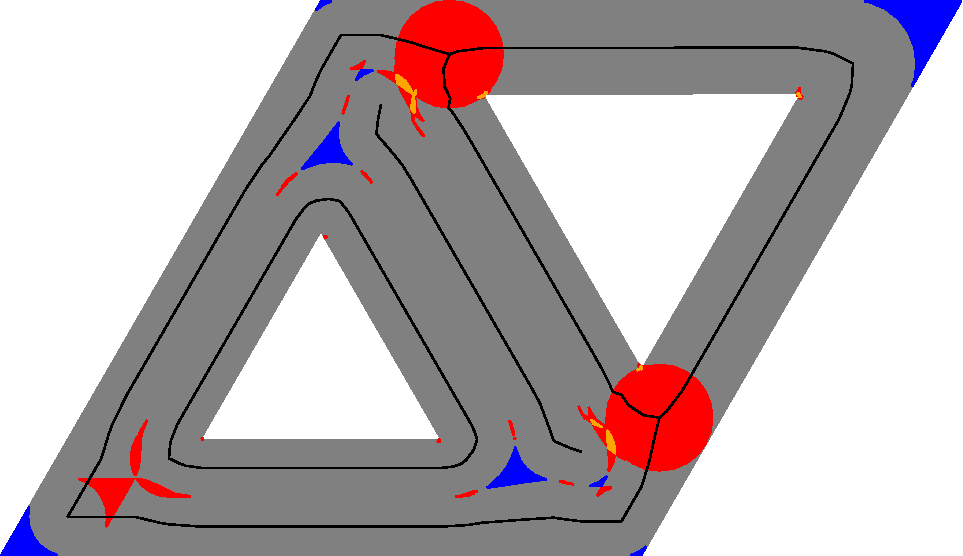
\includegraphics[width=\columnwidth]{sources/method/polyline_reduction_unreduced.pdf}
\caption{No reduction}
\end{subfigure}
\begin{subfigure}{0.45\figwidth}\centering
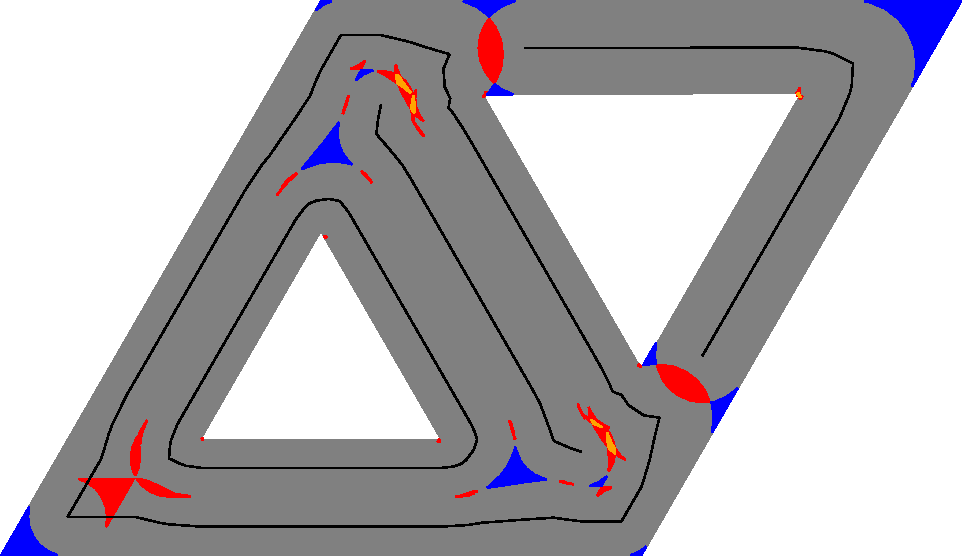
\includegraphics[width=\columnwidth]{sources/method/polyline_reduction_reduced.pdf}
\caption{Reduction}
\end{subfigure}
\caption{
Reducing polyline toolpaths away from intersections in order to prevent overextrusion.
Toolpath locations in black, underextrusion in blue, overextrusion in red and orange and normal extrusion in grey.
Intersections result in overextrusion, so we remove parts of the polylines at intersections.
}
\label{polyline_reduction}
\end{figure}



























































